\begin{refsegment}
\chapter*{De l'information au savoir}
\markboth{Introduction --- De l'information au savoir}{Introduction --- De l'information au savoir}
\addcontentsline{toc}{chapter}{Introduction --- De l'information au savoir}
Avec l'avènement des outils informatiques, la quantité d'information publiée ne cesse d'augmenter. Cette abondance de données disponibles rend plus difficile la gestion de l'information. Une des premières personnes qui a évoquée cette problématique d'explosion de l'information, est Frank Fremont-Smith directeur de l'institut Américain des Science Biologiques,  en \citeyear{fremont61}  \cite{fremont61}. Cette problématique est toujours d'actualité. Par exemple depuis 2012, chaque année, plus de 2,8 millions de documents scientifiques sont publiés  \cite{oecd2016} . Face à cette arrivée massive de savoir, la vérification et le croisement de toutes les publications n'est plus possible.

De plus, une partie non négligeable de ces documents scientifiques traite de thématique impliquant un très grand nombre de données. Ainsi, à ce nombre conséquent de publications s'ajoute une quantité de données importantes et très hétérogènes.

Au regard de cette problématique, comment mettre en place une démarche scientifique pour vérifier nos savoirs ?

Une méthode utilisée jusqu'alors, implique la vérification des théories par la mise en place d'expériences répétées. Cette méthodologie basée sur l'expérimentation permet de vérifier une hypothèse par des observations. L'expérimentation doit être menée de manière à que les conséquences étudiées soient liées de façon certaine à leur cause.

Il est important de rappeler que cette méthodologie a joué et joue toujours un rôle important dans les découvertes scientifiques. Cette méthode passe dans un premier temps par la formulation d'une hypothèse. Les différents acteurs de l'expérience sont déterminés. Puis dans un second on établit le plan de l'expérience, pour terminer enfin sur l'évaluation des résultats obtenus. Afin de conforter les résultats, l'expérience est répétée. Ce processus permet d'apporter les éléments de confiance et d'impartialité nécessaires pour vérifier une théorie. Toutefois la méthodologie expérimentale s'avère souvent plus longue et plus onéreuse que les méthodes basées sur des prédictions In-silico. 

\note{Dès l'antiquité, Aristote (384 - 322 av. J.-C.) décrit la nécessité d'expliquer les causes par l'utilisation de conséquences liées et avérées. Mais la première personne reconnue d'avoir utilisée cette méthodologie est Alhazen (965 - 1039). A travers son traité \citetitle{Alhazen1572}, il présente par des méthodes expérimentales que la lumière voyage en ligne droite. La découverte de cette loi physique est exceptionnel pour l'époque.}

Les méthodes basées sur le calcul informatique prennent de plus en plus d'importance. Elles sont facilement réutilisables, rapides et capables de traiter un très grand nombre d'informations. Ces méthodes sont développées en utilisant un jeu d'information déterminé au départ. Une fois que les résultats de la méthode sont validés, nous pouvons rechercher un algorithme capable de généraliser et d'apporter une solution globale au problème. Rien ne garantit que les informations fournies par la suite respectent le cadre théorique posé par l'algorithme. C'est pourquoi les résultats obtenus sont considérés comme des prédictions. Ces résultats n'ont pas le même degré de “certification” que ceux obtenus par une observation empirique.

En conséquence, tant les prédictions informatiques que les hypothèses émises par l'Homme devraient, dans l'idéal être vérifiées par une approche expérimentale. Afin de minimiser le nombre d'expérimentations, est-il intéressant de valider ou non des théories par comparaison de ce que l'on s'attends à obtenir vis à vis de ce que l'on prédit ?

Avec l'essor de ces nouvelles technologies, la barrière entre information et savoir devient de plus en plus floue.

\note{
    L'origine du mot science, vient du latin \textit{"scientia"} désignant le savoir.
    
    La connaissance est propre à une personne. À contrario le savoir est transmissible.
    
    De nombreuses langues, comme l'anglais ne possède pas de mot pour différencier savoir et connaissance. En effet, dans les deux cas on utilise \textit{"knowledge"}. Afin de marquer la nuance, on retrouve l'expression \textit{"certified knowledge"} pour le savoir et \textit{"learning by doing"} pour la connaissance.
}


Est-il possible de réunir les observations issues de méthodologies \textit{in silico} et celles issues de l'expérimentation en laboratoire autour d'un modèle théorique ?

Cette question nous amène à réfléchir à la représentation puis la validation des théories. En effet, comment évaluer des théories partiellement observées ? Mais également comment gérer les observations contradictoires ?

Apporter une méthode à cette vaste problématique permettrait de valider nos savoirs, d'identifier les concepts non observés et de caractériser les concepts contradictoires. Représenter ce savoir c'est également faciliter les échanges entre les différents domaines scientifiques.

\citation{La séparation des savoirs, la spécialisation en domaine isolé nuit considérablement au développement de la recherche.}{Jacques Le Goff}[Le Monde de l'éducation - mai 2000]

\change{Trop vulgarise}{David Vallenet}
Ce constat se vérifie en biologie notamment avec l'avènement des séquenceurs nouvelles générations. Le séquençage des organismes est devenu peu couteux et rapide. Ainsi la communauté scientifique a initié de vastes projets de séquençage de génomes qui visent à déterminer la séquence d' \gls{ADN} des organismes . Ces projets permettent d'avoir le code génétique, également nommée séquence \gls{ADN}. Cette chaîne \gls{ADN} peut être composée de quelques milliers à plusieurs centaines de millions de paires de bases nucléiques. Selon l'ordonnancement des bases nucléotidiques, des régions appelées gènes, procurent des fonctionnalités à l'organisme. Ainsi, L'\gls{ADN} est un point de départ pour l'étude et la compréhension des fonctionnalités inscrites dans le vivant.


\begin{shadedfigure}
    \centering
    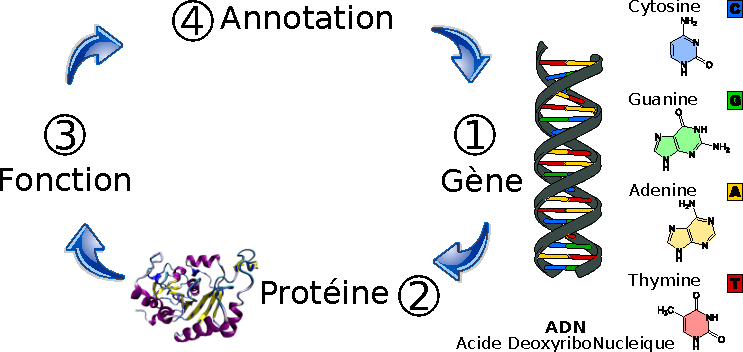
\includegraphics{img/simple_annotation_process.pdf}
    \caption{Vue globale du gène à l'annotation }
    \label{fig:glob_annotation}
\end{shadedfigure}

Des outils bio-informatiques analysent ces séquences afin de prédire les régions géniques et leurs fonctions dans l'organisme (voir \cref{fig:glob_annotation}). Selon les organismes, le nombre de gènes varie de quelques milliers à plusieurs dizaines de milliers de gènes. Ainsi, parmi le million voire milliard de paire de base d'\gls{ADN}, il faut identifier tous les gènes. Par conséquent, l'expertise humaine d'un génome est un défi en soi. Ces recherches se sont intensifiées et complexifiées, notamment avec la mise en place du projet d'étude de 100 000 génomes d'organismes pathogènes \cite{100kfoodborne}, ou encore l'analyse des eco-systèmes poly-microbiens présents sur l'Homme \cite{hmp}.

Pour se faire des outils bio-informatiques ont automatisé le traitement de l'information issue des séquenceurs afin de traiter un nombre d'organismes toujours plus grand. Ces outils, alimentés continuellement en nouveaux génomes, ont amplifié le déluge d'information. Dans le domaine de l'annotation fonctionnelle, moins d'un pour cent des données ont pu être vérifiées (au regard des statistiques publiées par UniProt et SwissProt en 2017 \parencites{uniprot_stat}{expasy_stat} ). Ce fossé entre information de confiance et prédiction s'accélère car il est plus rapide de produire de l'information que de la vérifier.

Or les prédicteurs automatiques de la fonction biologique des gènes ne sont pas fiables. En effet, 30\% des annotations fonctionnelles seraient incorrectes, voire 80\% dans certaines familles de protéines \parencites{devos2001intrinsic}{schnoes2009annotation}. Ces séquences incorrectement annotées sont ensuite propagées dans les bases de connaissances.

Une des méthodes d'assignation de fonction de gène, consiste à inférer une annotation provenant d'un gène connu à toutes les séquences similaires. En effet, il est supposé que l'évolution des produits des gènes sont sous pression de sélection afin de préserver leur fonction. L'ensemble des fonctions d'un organisme permet à ce dernier d'être adapté à son environnement. Étant donné qu'une modification d'un acide aminé impliqués dans la fonction peut potentiellement entrainer la perte de l'activité biologique. Et par conséquent mettre en péril les capacités de survit de l'organisme. Ces régions d'acides aminées devraient faiblement variées d'un point de vue physico-chimiques. Toutefois l'assimilation de proche en proche des fonctions biologiques tend à surestimé les propriétés biologiques d'une séquence. Car les séquences faussement annotées avec une fonction se retrouvent parmi les autres. Par conséquent, elles sont potentiellement utilisées, afin de propager une fonction d'un autre gène considéré similaire, détériorant un peu plus la qualité des bases de données.

L'objectif de l'annotation des fonctions géniques est de fournir un catalogue des capacités moléculaires et/ou biochimiques dont est pourvu un organisme. Ce catalogue permet de mieux comprendre le vivant. Cependant le processus d'annotation, produit et amplifie l'assignation de fonctions erronées à de nouveaux gènes et entraîne l'incapacité à utiliser ces prédictions sans prendre un risque. Le catalogue de fonctions géniques est en effet utilisé par la suite dans de nombreux domaines, comme l'étude des voies métaboliques, la biologie des systèmes, la classification des gènes essentiels et autres\ldots~Cette problématique impacte notre compréhension du vivant et notre capacité à l'étudier, remettant en cause tout le processus d'annotation des gènes utilisés jusqu'alors.

Face à cette problématique des approches variées ont été développés. On distingue les systèmes d'annotations automatiques à base de règle, reprenant le raisonnement appliqué par les bio-curateurs, comme le projet HAMAP \cite{lima2009hamap}. Ces règles sont généralement basées sur la séquence génomique et la taxonomie de l'organisme. Elles peuvent être créées par un bio-curateur ou par des outils d'apprentissage \cite{uniprot2011ongoing}.

On retrouve également les systèmes de reconstruction des voies métaboliques \cite{karpe2011pathway}. Ces méthodes utilisent des génomes complétement séquencés et bien annoté pour décrire des cascades de réactions amenant à un composé d'intérêt biologique.  Cette successions de réactions met en lumière un chemin à dans le réseaux de réactions, d'où le terme anglais "pathway" pour décrire un chemin qui amène à un objectif biologique. Par la suite, ces voies métaboliques identifiées sont proposées pour d'autres organismes dont l'annotation est partielles. Certains objectifs biologiques vont apparaître manquant au regards des prédictions sur les capacité métaboliques de l'organisme. Ces réseaux de concept forment un graphe de connaissance, spécifique de l'organisme. Ainsi, des fonctions marquées comme manquantes, à la réalisation de voie métabolique, sont suggérées aux bio-curateurs.

Les méthodes à base de règles automatisent l'annotation fonctionnelle par l'utilisation de règles liées à la biologie de l'organisme et non plus uniquement par une prédiction \textit{in silico}. Les méthodes, utilisant la représentation des connaissances biologiques, contextualisent les prédictions. De plus, elles permettent de suggérer des annotations fonctionnelles ne pouvant pas être détectées par les prédicteurs usuels. Toutefois, le travail de curation des annotations par un bio-curateur est nécessaire mais considéré comme fastidieux, laborieux et source d'erreur. Il apparaît nécessaire de fournir un assistant à la curation des fonctions géniques.

\section*{La démarche suivie dans cette thèse}

Mon travail de recherche s'est ouvert à de nombreuses disciplines afin d'apporter une méthode d'expertise des observations vis-à-vis du savoir, en biologie. En effet, la complexité du problème, nécessite l'intervention de concepts provenant de la logique, la représentation des connaissances, la théorie des graphes, la bio-informatique et le métabolisme. Ainsi, j'ai étudié ces différents domaines, décrypté le jargon, recherché les méthodes semblant avoir une application. Puis, je les ai combinées dans le but d'obtenir une méthode fiable et rapide.

Certaines voies furent des impasses, d'autres n'avaient pas encore de solution. À travers ces quelques chapitres je vous livrerai les notions et mon expérience sur ces différents domaines.

Cette thèse débute avec une problématique biologique \textit{"Comment guider et faciliter le travail des bio-curateurs, lors des étapes de l'annotation fonctionnelle ?"}. Pour cela, on souhaitait reprendre un prototype de vérification de la cohérence globale de l'annotation. En effet, l'équipe HELIX dirigé par \textit{Alain Viari} a travaillé sur une telle question. Leur projet a abouti à un raisonneur nommé HERBS. Cet outil permet de déterminer les concepts biologiques attendues et correctement prédits des autres concepts. Nous devions donc étendre ces fonctionnalités afin de prendre en compte l'incertitude et la contradiction. À ce moment nous pensions que le travail consistait à récupérer les méthodes logiques, puis de les adapter à la biologie, puis mettre à jour l'outil. Or à aucun moment, nous nous doutions que certaines problématiques de la logique, étaient toujours ouvertes. En effet, la logique a ses limites, notamment lorsque l'on travaille avec des concepts, dont certains peuvent prendre des états ni-vrai-ni-faux. Ou encore, lorsque l'on souhaite raisonner sur des ensembles d'ensemble. Comme je l'ai compris plus tard, le monde de la logique a été rythmé par des faits marquants comme le paradoxe de \textit{Russell}. Tel un historien, je me suis retrouvé dans les grandes problématiques de la logique moderne. Ainsi j'ai suivi les traces, de \textit{Platon} avec les bases de la logique classique, \textit{Bertrand Russell} pour les ensembles, \textit{Jan Łukasiewicz} et le principe de tiers exclu, \textit{Nuel Belnap} et la logique à quatre valeur.

\note{Le paradoxe de Russell démontre que si un ensemble est membre de lui-même, alors par définition il ne peut être un membre de lui-même. Mais s'il n'est pas un membre de lui-même, alors il est un membre de lui-même.
    
    Le paradoxe du barbier image une telle situation. Imaginer, Le conseil municipal d'un village vote un arrêté municipal qui enjoint à son barbier (masculin) de raser tous les habitants masculins du village qui ne se rasent pas eux-mêmes et seulement ceux-ci.
    
    Le barbier, qui est bien un habitant du village, n'a pas pu respecter cette règle car :
    \begin{itemize}
        \item S'il se rase lui-même, il enfreint la règle, car le barbier ne peut raser que les hommes qui ne se rasent pas eux-mêmes ;
        \item S'il ne se rase pas lui-même - qu'il se fasse raser ou qu'il conserve la barbe - il est en tort également, car il a la charge de raser les hommes qui ne se rasent pas eux-mêmes.
    \end{itemize}
}

D'autre part, il apparut très tôt la nécessité de représenter le savoir, dans un modèle générique. Permettant ainsi d'avoir un modèle, utilisable pour le plus grand nombre d'entrepôts de données. Cette recherche commença par les travaux de John F. Sowa sur la représentation des connaissances ( \citeyear{sowa92,sowa99}).

Le défi est de représenter des connaissances, sans a priori sur la représentation des données dans les entrepôts de données. Pour cela, un travail de structuration des concepts et de classification de leurs relations a été mené. Ce travail m'a amené à étudier la logique de description \cite{baader2003description}. Concrètement ce domaine de recherche permet de faire le lien entre l'intelligence artificielle et la représentation du savoir. L'étude portée sur cette représentation du savoir est un sujet très dynamique, avec l'essor du \textit{Web Semantic}. Cette thématique se consacre à l'étude de la nature des concepts, de leur relations, mais également de leur existence définissant par la même l'ontologie.

Dans l'objectif de cartographier notre savoir en Biologie, un consortium international s'est créé : \textit{\gls{GO}} (voir G. O. Consortium
et al \citeyear{go2001,go2004}). Les concepts sont classifiés parmi trois catégories distinctes (i) les fonctions moléculaires, (ii) les processus biologiques et (iii) les composants cellulaires. Les concepts sont appelés des GO termes. Les relations entre les termes porte des étiquettes pour exprimer les notions de composition et de type \cref{fig:go_relation}. Ces descriptions de connaissances sont effectuées avec un langage contrôlé.  C'est à dire que le vocabulaire et la grammaire est restreinte, afin de réduire l'ambiguïté et donc la complexité des textes. Un tel langage permet à un programme informatique de comprendre une phrase. Ainsi cet ensemble de mot peut être utilisé pour vérifier la cohérence du texte. Ou encore un utilisateur peut effectuer des interrogations sur l'ensembles des connaissances décrites.

Figure ici: ftp://ftp.geneontology.org/pub/go/www/GO.ontology.relations.shtml


La structure des données répondait à nos besoins. Cependant le lien entre les termes d'une catégorie avec une autre n'était pas fourni. Par exemple on ne peut pas relier des processus biologiques à des fonctions moléculaires. Des projets comme \cite{AdditionalGO2006} parviennent partiellement à couvrir les liens  entre les termes des différentes catégories.

Toutefois, un nombre trop important de relation restait manquante. Pour cette raison, j'ai mis au point une structure de concept avec toutes les notions nécessaires afin de représenter nos connaissances. Cette structure sera le support d'inférence des observations biologiques. L'objectif étant de vérifier l'existentialité de nos connaissances sur chaque organisme.

Tout au long de mon travail de recherche j'ai été confronté à des limites. Si bien que des solutions nouvelles devaient être inventées. La problématique d'apparence simple s'est révélée plus complexe. Ainsi, j'ai dû rechercher des notions dans des domaines "éloignés" de la bio-informatique comme \textit{la Logique}. Établir un modèle générique afin de représenter toute sorte de données, même celle auxquelles je n'aurais pas pensé ! J'ai également mis en place des méthodes permettant d'intégrer un volume de donnée conséquent tout en étant capable de fournir un résultat dans un temps raisonnable. Ce travail m'a demandé de dépasser les paradoxes de la logique afin de l'étendre aux notions d'inconnu et de contradiction. De sorte que la méthode finale puisse proposer des annotations manquantes, mettre en lumière les contradictions, de vérifier les prédictions \textit{In-Silico} avec les expectations biologiques, explorer les capacités métaboliques de tout organisme.

Pour cela, la suite de cette thèse commence par une présentation des concepts métaboliques et de leurs représentations informatiques. Puis, les liens entre génome et métabolisme seront détaillés. Pour continuer sur les données biologiques dont nous disposons. Suivi par des notions sur la \textit{Logique} et l'\gls{IA}. On continuera par les systèmes experts, utilisé pour résoudre des problèmes biologiques. Ceci, introduira le début de GROOLS. Mais également, les problématiques qui étaient restés ouvertes jusqu'alors. Afin de parvenir aux notions de raisonnement descriptif avec la méthode mise en œuvre dans GROOLS, cette thèse se termine par la présentation des résultats et les pistes de recherches envisagées.


\subbibliography
\end{refsegment}